\chapter{Measurements}
\section{Human Expertise Test}\label{6_sec:expertise_test}
In order to better grasp the audio quality, directivity and beam steering of the Audio-Beamformer, a human expertise test was conducted. The device was shown to 17 people in different test settings.   
\subsection{Test Setup}
To fully test the capabilities of the device a free standing location was chosen so that the reverberation could be neglected. In Figure \ref{6_fig:measurement_setup_final} the five different points (A, B, C, D, E) where the measurements took place are shown. These points are all in a distance of ten meters to the loudspeaker. The points A and E are at an angle of 30 degrees and B and D are at 15 degrees. The point C is directly in front of the device.

\bigskip
\begin{figure}[h!]
    \centering
    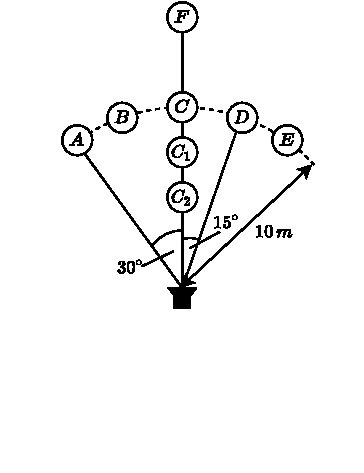
\includegraphics[width=8cm, trim=0mm 22mm 0mm 0mm]{images/6_Measurements/MeasurementSetup.pdf}
    \caption{Measurement Setup Final Tests}
    \label{6_fig:measurement_setup_final}
\end{figure}
\newpage

\subsection{Audio Quality}
To evaluate the audio quality, a rating scale has been developed, based on the Swiss grading system. This is shown in Table \ref{6.1.2_tab:audio_quality}.
\begin{center}
\begin{table}[h!]
\centering
\begin{tabular}{ |m{2.1cm}|m{2.1cm}|m{2.1cm}|m{2.1cm}|m{2.1cm}|m{2.1cm}|}
  \hline 
  1 & 2 & 3 & 4 & 5 & 6\\ 
  \hline
 Completely unrecognizable audio, very distorted and noisy & Hardly anything can be recognized, noise and distortion are dominant & Mostly recognizable audio, distortion and noise clearly audible &  Acceptable hearing experience, speech recognizable without effort & Enjoyable hearing experience, appropriate for daily use &  Outstanding Hi-Fi audio quality, no noise audible \\
 \hline
\end{tabular}
\caption{Audio Quality Grading Scale}
\label{6.1.2_tab:audio_quality}
\end{table}
\end{center}

\subsubsection{Measurements}
\begin{enumerate}
    \item General Audio Quality \\
    To test the general audio quality, music and speech was played. All settings were set to default.
    \begin{center}
     \begin{table}[ht]
    \centering
    \begin{tabular}{ |c|c|c|}
      \hline 
      Test & Average & Variance \\ 
      \hline
     Music quality & 4.2 & 0.46 \\
     \hline
     Speech quality & 4.5 & 0.38 \\
     \hline
    \end{tabular}
    \caption{Audio Quality Score}
    \label{6.1.2_tab:music_audio_quality}
    \end{table}   
    \end{center}
    \item Equalizer \\
    For the second test, the equalizer was changed and the music quality of each preset was tested. The equalizer \textit{Main} was not specifically tested but it is the default equalizer and is mentioned in Table \ref{6.1.2_tab:music_audio_quality_eq} as a comparison.
     \begin{center}
     \begin{table}[ht]
    \centering
    \begin{tabular}{ |c|c|c|}
      \hline 
      Test & Average & Variance \\ 
      \hline
     No equalizer & 4.1 & 0.67 \\
     \hline
     Equalizer: \textit{Lowcut 300Hz} & 4.25 & 0.60 \\
     \hline
     Equalizer: \textit{Sharp} & 4 & 0.66 \\
     \hline
     Equalizer: \textit{Main} & 4.2 & 0.46 \\
     \hline
    \end{tabular}
    \caption{Audio Quality of different Equalizers}
    \label{6.1.2_tab:music_audio_quality_eq}
    \end{table}   
    \end{center}
    \item Modulation Type \\
    At last, the audio quality of the two modulations types \acrshort{am} and \acrshort{mam} were compared. The other settings were again set to default.
    \begin{center}
     \begin{table}[ht]
    \centering
    \begin{tabular}{ |c|c|c|}
      \hline 
      Test & Average & Variance \\ 
      \hline
     \acrshort{am} & 3.9 & 0.40 \\
     \hline
     \acrshort{mam} & 4.4 & 0.34 \\
     \hline
    \end{tabular}
    \caption{Audio Quality of different Modulation Types}
    \label{6.1.2_tab:music_audio_quality_mod}
    \end{table}   
    \end{center}
\end{enumerate}
A more detailed overview of the quality measurements can be seen in Figure \ref{6_fig:box_plot_quality}.
\begin{figure}[h!]
    \centering
    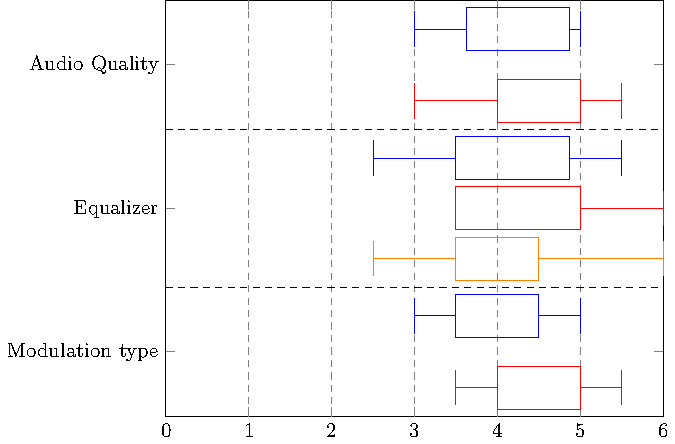
\includegraphics[width=0.7\textwidth]{images/6_Measurements/BoxPlotQuality.pdf}
    \caption{Audio Quality Box-Plot}
    \label{6_fig:box_plot_quality}
\end{figure}

\subsubsection{Evaluation}
The general audio quality test turned out well, as both music and speech were rated on average better than an acceptable hearing experience. Especially the audio quality of speech surprised us and showed that this could be an important use case. In the equalizer test all results turned out to be about the same and statistically show no significant difference between them. We think with more time and more testing better and more impressive equalizer settings can be found and these results can be improved on. 
The modulation type test painted a strong picture that \acrshort{mam} modulation is the way to go. 
Overall, we are very pleased with these results and think a real alternative to conventional loudspeakers can be created with further improvements. 
\newpage

\subsection{Audio Volume}
To evaluate the beam steering capability and overall directivity, a grading system was developed. This is shown in Table \ref{6.1.3_tab:audio_volume}.

\begin{center}
\begin{table}[h!]
\centering
\begin{tabular}{ |m{2.2cm}|m{2.2cm}|m{2.2cm}|m{2.2cm}|m{2.2cm}|}
  \hline 
  -4 & -3 & -2 & -1 & 0\\ 
  \hline
Nearly nothing audible, not noticeable volume level &	Noticeable if background is quiet (no one is talking) &	Strongly noticeable volume level, even with background noise (speech) &	Clearly audible volume level & Very present volume level, strongly dominates background noise
\\
 \hline
\end{tabular}
\caption{Audio Volume Grading Scale}
\label{6.1.3_tab:audio_volume}
\end{table}
\end{center}

\subsubsection{Measurements}
Due to the absolute value of the volume being very objective, the results of each individual test was normalized to be between 1, very loud, and zero, nothing audible. This means that the following list of test results says nothing about the absolute value of the Audio-Beamformer.
\begin{enumerate}
    \item Directivity \\
    To test the directivity, the test person had to rate the volume at every point (A, B, C, D and E). Once with no window applied and once with the Dolph-Chebyshev window, which should, in theory, generate a more directive beam.
    \begin{center}
     \begin{table}[h!]
    \centering
    \begin{tabular}{ |c|c|c|c|c|c|c}
      \hline 
      Test & A & B & C & D & E \\ 
      \hline
     No window & 0.34 & 0.57 & 1 & 0.66 & 0.43 \\
     \hline
     Dolph-Chebyshev & 0.32 & 0.5 & 1 & 0.54 & 0.34 \\
     \hline
    \end{tabular}
    \caption{Audio Directivity}
    \label{6.1.2_tab:music_audio_volume_directivity}
    \end{table}   
    \end{center}
    \item Beam Steering \\
    To test the beam steering, two different tests were carried out.
    \subitem Point C\\
    In the first test, the test person stood on Point C and the beam was steered to an angle of 0, 15 or 30 degrees. This was testes with no window and the Dolph-Chebyshev window.
    \begin{center}
     \begin{table}[h!]
    \centering
    \begin{tabular}{ |c|c|c|c|}
      \hline 
      Test & $0^\circ$ & $15^\circ$ & $30^\circ$ \\ 
      \hline
     No window & 0.98 & 0.8 & 0.83 \\
     \hline
     Dolph-Chebyshev & 1 & 0.72 & 0.70 \\
     \hline
    \end{tabular}
    \caption{Beam Steering Point C}
    \label{6.1.3_tab:music_audio_volume_steering_c}
    \end{table}   
    \end{center}
     \subitem Point A\\
    For the second test, the test person stood on Point A and the beam was steered to an angle of 0, 15 or 30 degrees. This was testes with no window or the Dolph-Chebyshev window.
    \begin{center}
     \begin{table}[h!]
    \centering
    \begin{tabular}{ |c|c|c|c|}
      \hline 
      Test & $0^\circ$ & $15^\circ$ & $30^\circ$ \\ 
      \hline
     No window & 0.55 & 0.71 & 0.96 \\
     \hline
     Dolph-Chebyshev & 0.38 & 0.51 & 1 \\
     \hline
    \end{tabular}
    \caption{Beam Steering Point A}
    \label{6.1.3_tab:music_audio_volume_steering_A}
    \end{table}   
    \end{center}
\end{enumerate}
\subsubsection{Evaluation}
The directivity test showed that already at around $\pm 30^\circ$ the sound is almost only noticeable if the background is quiet. One can also see that the Dolph-Chebyshev window is, as expected, more directive. From the beam steering tests one saw that, especially with no window it is very difficult to keep the point directly in front of the speaker quiet. This is in our opinion mainly due to the inherit directivity of the loudspeaker. The second test, at point A, shows that the beam steering works as expected.
\newpage

\section{Ultrasound Measurements}\label{6_sec:ultrasonic}
As an addition to the human expertise test, a measurement series was carried out. Because we had no sound chamber at our disposal we had to carry out these measurements outside. But due to the surrounding noise, a measurement in the audible spectrum was impossible so all the measurements where carried out only with the carrier. As a result of this, and the difficulties of sound measurement without am ideal setup, measurement device and location these measurements have to be viewed with a pinch of salt.
\subsection{Directivity}
The directivity of the ultrasound was measured with and without a window at 9 distinct points between $-30^\circ$ and $30^\circ$. The results of these measurements are shown in Figure \ref{6.2.1_fig:Directivity_measurements}.
\begin{center}
    \begin{figure}[h!]
        \centering
        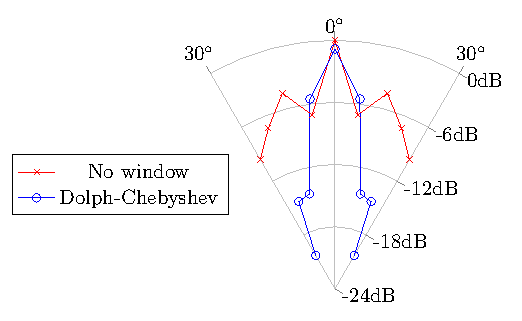
\includegraphics[width=0.5\textwidth]{images/6_Measurements/Polar_PlotDirectivity_Measurement.pdf}
        \caption{Directivity Measurements}
        \label{6.2.1_fig:Directivity_measurements}
    \end{figure}
\end{center}

\subsection{Beam Steering}
To measure the effects of the beam steering, the beam was once directed to $15^\circ$, as seen in Figure \ref{6.2.2_subfig:beamsteering_15}, and once directed to $30^\circ$, as seen in Figure \ref{6.2.2_subfig:beamsteering_30}. The dashed lines in both figures show the on the steered angle mirrored points to give a better feeling of how the beam looks. Due to the inherit directional nature of the loudspeaker, these dashed lines would in practice fall off a lot quicker than shown here. 
\begin{figure}[h!]
    \begin{minipage}{0.49\textwidth}
        \centering
        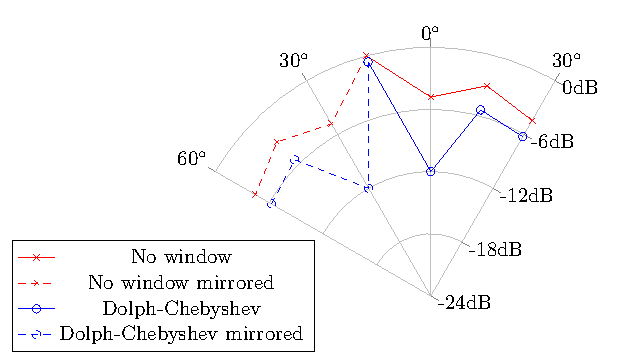
\includegraphics[width=\linewidth]{images/6_Measurements/Polar_PlotSteering_Measurement_15.pdf}
        \caption{Beam steered to 15$^\circ$}
        \label{6.2.2_subfig:beamsteering_15}
    \end{minipage}
    \begin{minipage}{0.49\textwidth}
        \centering
        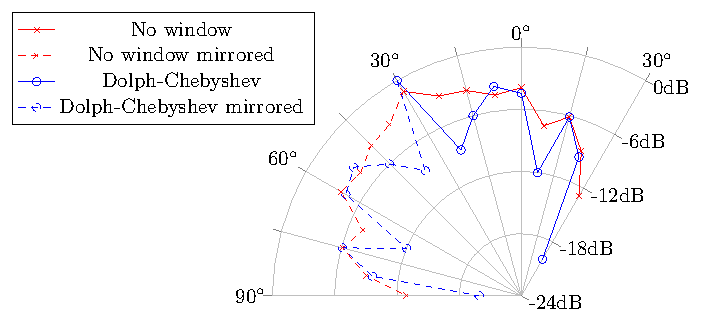
\includegraphics[width=\linewidth]{images/6_Measurements/Polar_PlotSteering_Measurement_30.pdf}
        \caption{Beam steered to 30$^\circ$}
         \label{6.2.2_subfig:beamsteering_30}
    \end{minipage}
\end{figure}

\subsection{Beam Focusing}
The beam focusing was tested on the Points C1 (7.5m), C2 (5m) and F (15m). The results of this are shown in Figure \ref{6_fig:beamforming_measurements}.
\begin{figure}[h!]
    \centering
    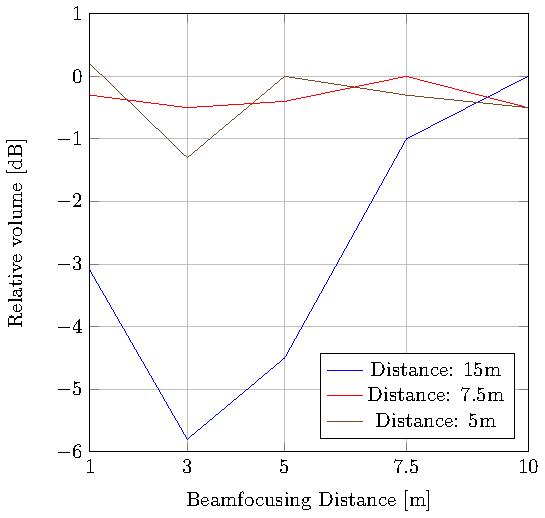
\includegraphics[width=0.4\textwidth]{images/6_Measurements/Beamfocusing.pdf}
    \caption{Beam Focusing Measurements}
    \label{6_fig:beamforming_measurements}
\end{figure}
\subsection{Evaluation}
As already said, due to the imperfect measurement setup these measurements have to be looked at critically. That said, the directivity and beam steering reflect the human expertise tests really well. In comparison to the calculations made in \ref{3_Parametric_array_Sec:Array_signal_processing} the measurements look similar, the main difference is the size of the side lobes, which in our measurements are a lot smaller than calculated. This is most likely due to the directivity of the transducers not being the their assumed sinc function, as shown in Figure \ref{5_fig:directivity_transducer}. 
The beam focusing, on the other hand seems to only work if the distance to the loudspeaker is big enough. To verify further tests have to be made under more ideal conditions. 
\newpage

\section{Transducer Measurements}
To get a better feeling for the transducers and to see how they behave under different circumstances, several measurements where taken. 
\subsection{Frequency Response}\label{6_sec:Frequency_response}
To be able to design more accurate equalizers, the sound pressure level output at each frequency between 22.5\,kHz and 55\,kHz was measured and is shown in Figure \ref{6_Measurement_fig:Transducer_FR}. But again due to no access to a sound chamber these measurements have to be looked at critically.
\begin{figure}[h!]
    \centering
    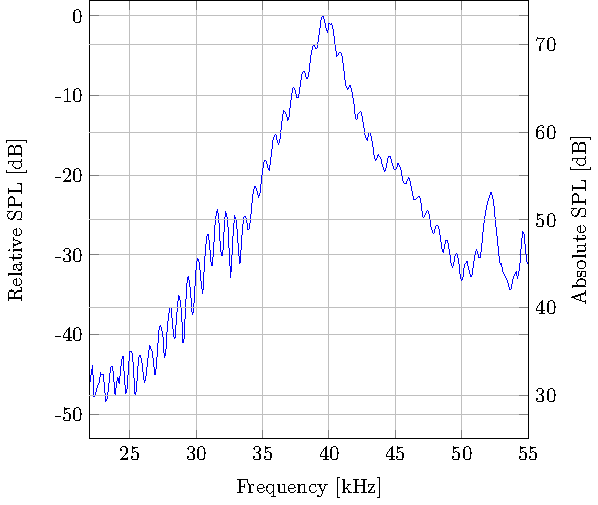
\includegraphics[width=0.5\textwidth]{images/6_Measurements/Transducer_Frequency_Respone.pdf}
    \caption{Frequency Response Transducer}
    \label{6_Measurement_fig:Transducer_FR}
\end{figure}
\subsection{Power Consumption}\label{6_subsec:Power_cons}
The power consumption of each of the 19 transducer lines is very important to access the output power of the loudspeaker. Over a $22 \, \Omega$ resistor in front of the transducer the current could be calculated. The voltage over the transducer and the voltage over the resistor was measured for 4 hours and it turned out that both these values were very constant. The voltage measured over the transducer was $U_T = 9.5 \,$V \acrshort{rms} and the voltage over the resistor $U_R = 1.78 \,$V \acrshort{rms}.
\subsection{Impedance Measurements}\label{6_subsec:impedance_measure}
To get information about the electrical side of the transducers, an impedance measurement was carried out with a series of 20 transducers. It was measured using a vector network analyser.
These measurements can be found in the Audio-Beamformer-software repository (Appendix \ref{Data Archive}).
\newpage